\chapter{Eksperymenty i analiza wyników}


\section{Przeprowadzenie eksperymentów i zbieranie danych}

Przeprowadzenie eksperymentów zostało wykonane na laptopie Dell z procesorem Intel Core i5-1135G7 z częstotliwością 2.40GHz i 16 GB pamięci RAM. Wybór tego sprzętu został podyktowany jego dostępnością oraz wystarczającymi parametrami technicznymi do wykonania zaplanowanych testów.

W procesie generowania danych wejściowych, takich jak grafy, przyjęto zastosowanie biblioteki igraph, która stanowi potężne narzędzie w dziedzinie analizy grafów. Biblioteka ta oferuje wszechstronne możliwości tworzenia, manipulowania oraz analizy grafów, co czyni ją popularnym wyborem wśród badaczy i praktyków zajmujących się analizą sieci oraz grafów. Zaawansowane funkcje igraph umożliwiają generowanie różnorodnych typów grafów, w tym grafów skierowanych i nieskierowanych, o różnych rozmiarach i strukturach. Dodatkowo, igraph dostarcza mechanizmy do manipulacji wierzchołkami oraz krawędziami grafu, co pozwala na elastyczne dostosowanie danych wejściowych do potrzeb konkretnego badania czy eksperymentu. 

Zdecydowano się generować dwa rodzaje grafów - Barabasi-Alberta i Erdos-Rényi'ego - w celu przeprowadzenia eksperymentów nad zróżnicowanymi właściwościami strukturalnymi. Ta strategia pozwala na badanie efektywności SMT-solverów w różnych warunkach oraz umożliwia pełniejszą analizę. 

Grafy Barabasi-Alberta są generowane na podstawie modelu preferencyjnego przyrostowego, zaproponowanego przez Alberta-László Barabási i Réka Albert w 1999 roku.

W tym modelu nowe wierzchołki dołączają się do grafu, preferując dołączanie do wierzchołków, które już mają wiele krawędzi, co prowadzi do powstania "hubów" lub wierzchołków o wysokim stopniu.
Parametr $m$ określa liczbę nowych krawędzi do dodania dla każdego nowego wierzchołka. W funkcji $\generategraph$ używamy losowej liczby z zakresu od $1$ do $10$ jako wartość $m$.

Grafy Barabasi-Alberta są często stosowane do modelowania sieci skomplikowanych, takich jak sieci społecznościowe, internetowe, czy biologiczne.

Grafy Erdos-Rényi'ego są generowane na podstawie modelu losowych grafów, zaproponowanego przez Paula Erdősa i Alfréda Rényiego w 1959 roku.
W tym modelu każda możliwa krawędź między wierzchołkami grafu ma jednakowe prawdopodobieństwo istnienia.
Parametry $n$ i $m$ określają odpowiednio liczbę wierzchołków i krawędzi grafu. W funkcji $\generategraph$ ustawiamy m na wartość równą $2 * n - \text{random.randint}(1, \frac{n}{2})$, co oznacza, że grafy typu Erdős-Rényi generowane są z różną gęstością krawędzi.
Grafy Erdos-Rényi'ego są często używane w badaniach nad teorią grafów, a także w symulacjach losowych procesów, takich jak transmisja informacji w sieciach komputerowych czy analiza przypadkowych struktur.

Funkcja $\generategraph$ służy do generowania dwóch typów nieskierowanych grafów, omówionych wyżej, o różnych rozmiarach z zakresu od 4 do 24 z krokiem co 2, oraz zapisywania ich w formacie listy krawędzi (edgelist) do odpowiednich plików tekstowych. 

\lstinputlisting[caption={Funkcja $\generategraph$}]{./codes/generate_graph.py}

Funkcja $\generatedigraph$ służy do generowania skierowanych grafów. Jest podobna do funkcji $\generategraph$, z wyjątkiem tego, że generuje ona skierowane krawędzie. 

\lstinputlisting[caption={Funkcja $\generatedigraph$}]{./codes/generate_digraph.py}

Funkcja $\appendweights$ została stworzona w celu przygotowania danych testowych do analizy efektywności solverów w rozwiązywaniu problemu Komiwojażera. Odczytuje ona zawartość każdego pliku linia po linii, przypisując wierzchołki źródłowe i docelowe każdej krawędzi do zmiennych s i t. Następnie generuje losową wagę dla każdej krawędzi w zakresie od 1 do 100. Ostatecznie funkcja zapisuje każdą krawędź wraz z jej wagą do pliku, nadpisując pierwotną zawartość pliku.

\lstinputlisting[caption={Funkcja $\appendweights$}]{./codes/append_weights.py}

Do generowania zestawów liczb całkowitych o różnych rozmiarach, przeznaczonych do eksperymentów nad problemem $\SubsetSum$ służy funkcja $\generatesets$. Zestawy te są tworzone w sposób losowy w zakresie od 5 do 55 liczb całkowitych, z krokiem co 5, korzystając z funkcji random.sample(range(1, n * 10), n). Funkcja random.sample() zwraca losowy podzbiór n elementów z zakresu od 1 do n * 10. Każdy zestaw liczb jest reprezentowany jako zbiór. Następnie funkcja zapisuje każdy wygenerowany zestaw liczb do pliku tekstowego o nazwie odpowiadającej rozmiarowi zestawu, gdzie każda liczba jest oddzielana spacją.

\lstinputlisting[caption={Funkcja $\generatesets$}]{./codes/generate_sets.py}


\section{Analiza zebranych danych i porównanie efektywności solverów}

\subsection{Wyniki dla Problemu ścieżki Hamiltona w grafie skierowanym}

\subsection{Wyniki dla Problemu ścieżki Hamiltona w grafie nieskierowanym}

\subsection{Wyniki dla Problemu maksymalnej kliki}

W badaniach nad problemem maksymalnej kliki dla grafów typu Barabási-Alberta, eksperymenty wykazały, że solver Z3 okazał się najszybszym spośród analizowanych. Obserwowano wyraźną tendencję wzrostową czasu wykonania wraz z rosnącą liczbą zmiennych, co potwierdzało złożoność obliczeniową problemu.

Obserwowano, że rozmiar maksymalnej kliki zwiększał się w sposób regularny, zazwyczaj o jeden wierzchołek, w miarę rosnącej liczby wierzchołków w grafie. Ta regularność wzrostu rozmiaru kliki jest charakterystyczna dla tego typu sieci, gdzie nowe wierzchołki preferują łączenie się z istniejącymi wierzchołkami o większym stopniu.

Na rysunku \ref{fig:3-barabasi-plot} przedstawiono wyniki eksperymentów dla danych grafów.

W przypadku ustawienia limitu czasu na 600 sekund, solver Yices nie był w stanie wykonać obliczeń dla grafów zawierających 16 wierzchołków, podczas gdy solver CVC5 osiągnął swoje ograniczenie na 18 wierzchołkach. Oznacza to, że Yices nie był w stanie znaleźć rozwiązania w przewidzianym czasie nawet dla grafów o stosunkowo niewielkim rozmiarze, podczas gdy CVC5 wykazał lepszą skalowalność, ale również osiągnął swoje ograniczenie dla większych grafów.

\begin{figure}[htbp]
	\centering
	\begin{minipage}{\textwidth}
		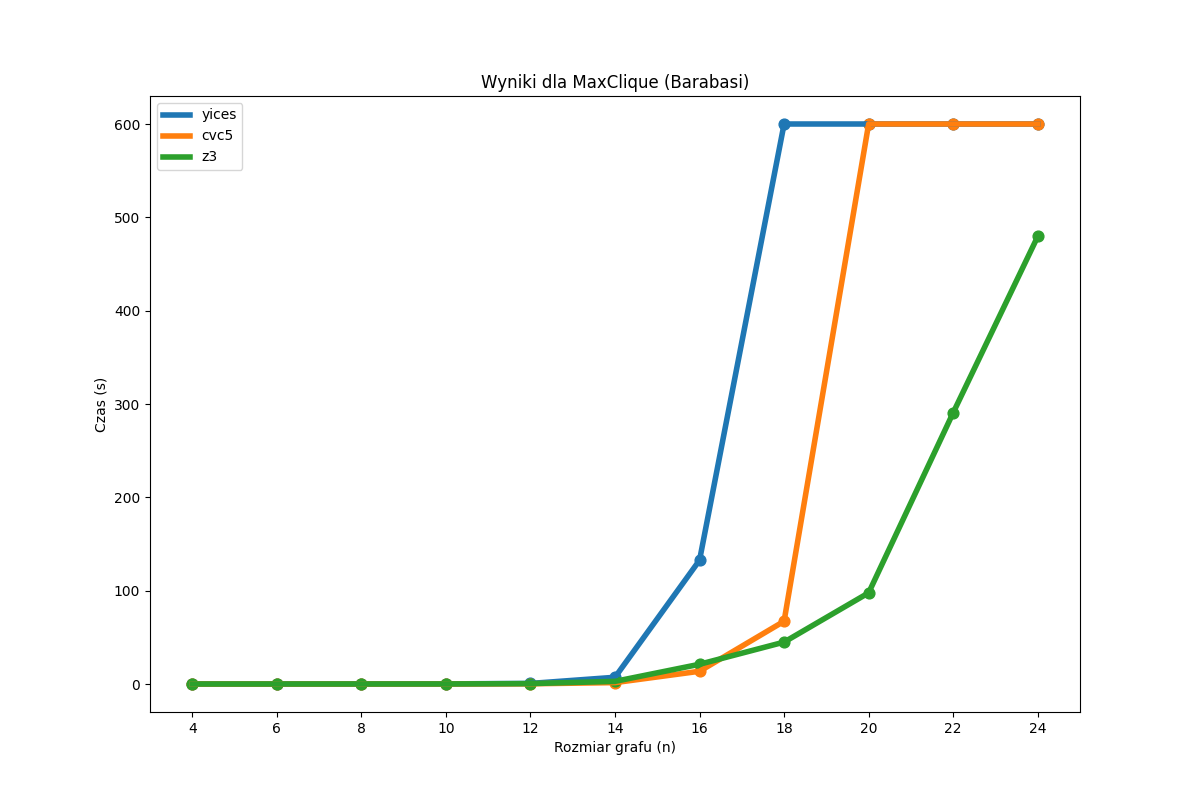
\includegraphics[width=\textwidth]{./figures/3-barabasi-plot.png}
		\caption{Wyniki eksperymentów dla grafów typu Barabási-Alberta.}
		\label{fig:3-barabasi-plot}
	\end{minipage}
\end{figure}

Eksperymenty dla grafów typu Erdős-Rényi'ego wykazały interesującą zależność czasu działania solverów od rozmiaru poszukiwanej kliki, szczególnie w przypadku braku istnienia kliki o zadanej wielkości. Im większy był rozmiar poszukiwanej kliki, tym dłużej zajmowało czasu na stwierdzenie, że problem jest niespełnialny. W takich sytuacjach, gdzie solver musiał sprawdzić większą liczbę możliwych kombinacji w poszukiwaniu niespełnialnego warunku, czas wykonania wzrastał wykładniczo wraz ze wzrostem rozmiaru poszukiwanej kliki.

Widoczne na rysunku \ref{fig:3-erdos-renyi-plot}, że rozmiar maksymalnej kliki nie podlegał takiej regularności, jak w grafach Barabási-Alberta, ponieważ struktura tych grafów opiera się na losowych połączeniach między wierzchołkami. W związku z tym, rozmiar maksymalnej kliki mógł się zmieniać losowo dla każdego kolejnego grafu. Dla pewnych konfiguracji, gdzie istniały większe kliki, czas potrzebny na znalezienie maksymalnej kliki był dłuższy, co można zaobserwować na wykresie, ponieważ w procesie rozwiązywania problemu, solver musiał uwzględniać większą liczbę wierzchołków i krawędzi, co prowadziło do wydłużenia czasu wykonania. Z3 nadal był najszybszym spośród badanych.

\begin{figure}[htbp]
	\centering
	\begin{minipage}{\textwidth}
		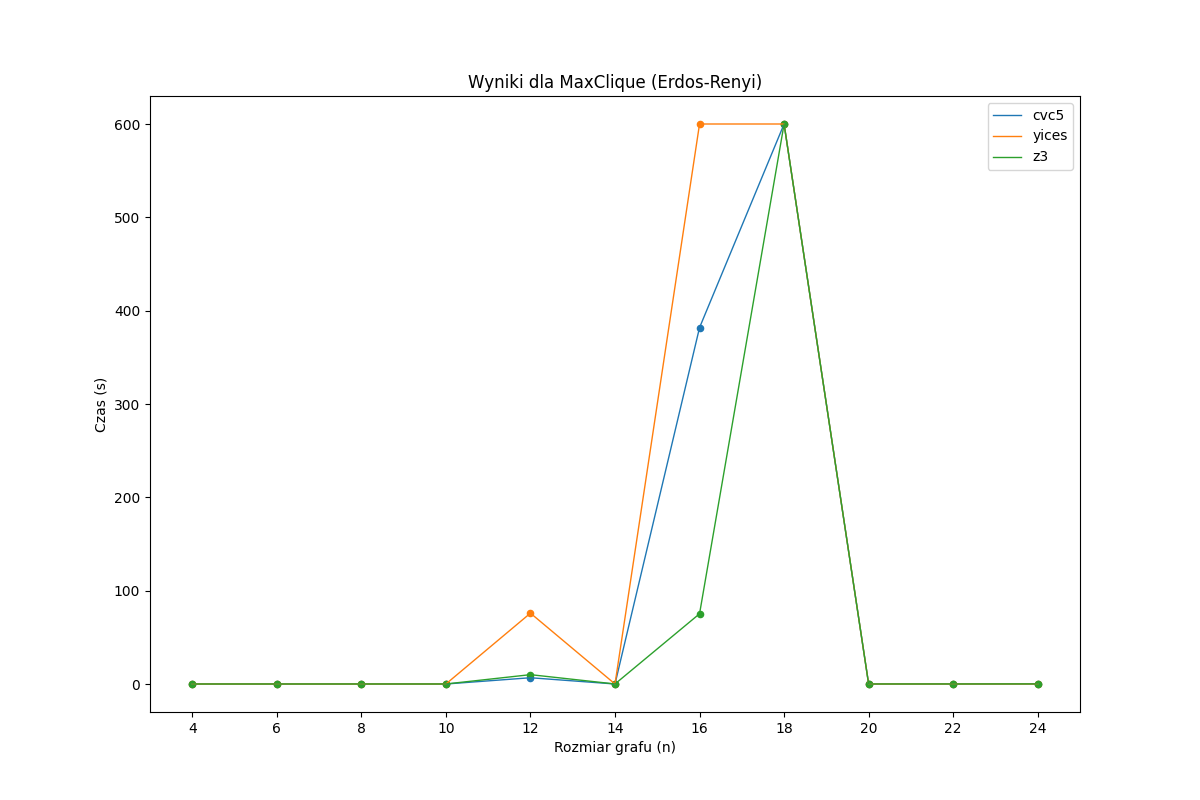
\includegraphics[width=\textwidth]{./figures/3-erdos-renyi-plot.png}
		\caption{Wyniki eksperymentów dla grafów typu Erdős-Rényi'ego.}
		\label{fig:3-erdos-renyi-plot}
	\end{minipage}
\end{figure}

Wnioskiem z tych eksperymentów jest, że czas działania solverów Z3, Yices i CVC5 zależy nie tyle od liczby wierzchołków, co od rozmiaru poszukiwanej kliki, zwłaszcza w przypadku braku istnienia kliki o zadanej wielkości. Dla przypadków, gdzie poszukiwana klika istniała, czasy działania były bardziej stabilne i niezależne od rozmiaru poszukiwanej kliki.


\subsection{Wyniki dla Problemu maksymalnego niezależnego zbioru}

W wynikach eksperymentów dla problemu maksymalnego niezależnego dla grafów Barabási-Alberta, obserwowano interesujące różnice w ich wydajności.

Na podstawie danych z wykresu \ref{fig:4-barabasi-plot} można stwierdzić, że zarówno Z3, jak i Yices wykazały podobnie szybkie reakcje, udzielając odpowiedzi w ciągu zaledwie 0.3 sekundy. Jednak warto zwrócić uwagę na ten fakt, że analizowane grafy miały małe rozmiary niezależnych zbiorów, z reguły zawierające 2-4 wierzchołki.

Natomiast CVC5, mimo że jest potężnym solverem SMT, napotkał znaczne trudności w rozwiązywaniu problemu dla większych instancji grafów. Już na 12 wierzchołkach CVC5 nie był w stanie udzielić odpowiedzi w określonym limicie czasu 600 sekund, szczególnie dla mniejszych wartości parametru $k$ (rozmiar zbioru). To znaczące opóźnienie w stosunku do Z3 i Yices jest interesującym spostrzeżeniem, co może sugerować, że CVC5 ma trudności w radzeniu sobie z tym konkretnym problemem w przypadku bardziej złożonych instancji.

\begin{figure}[htbp]
	\centering
	\begin{minipage}{\textwidth}
		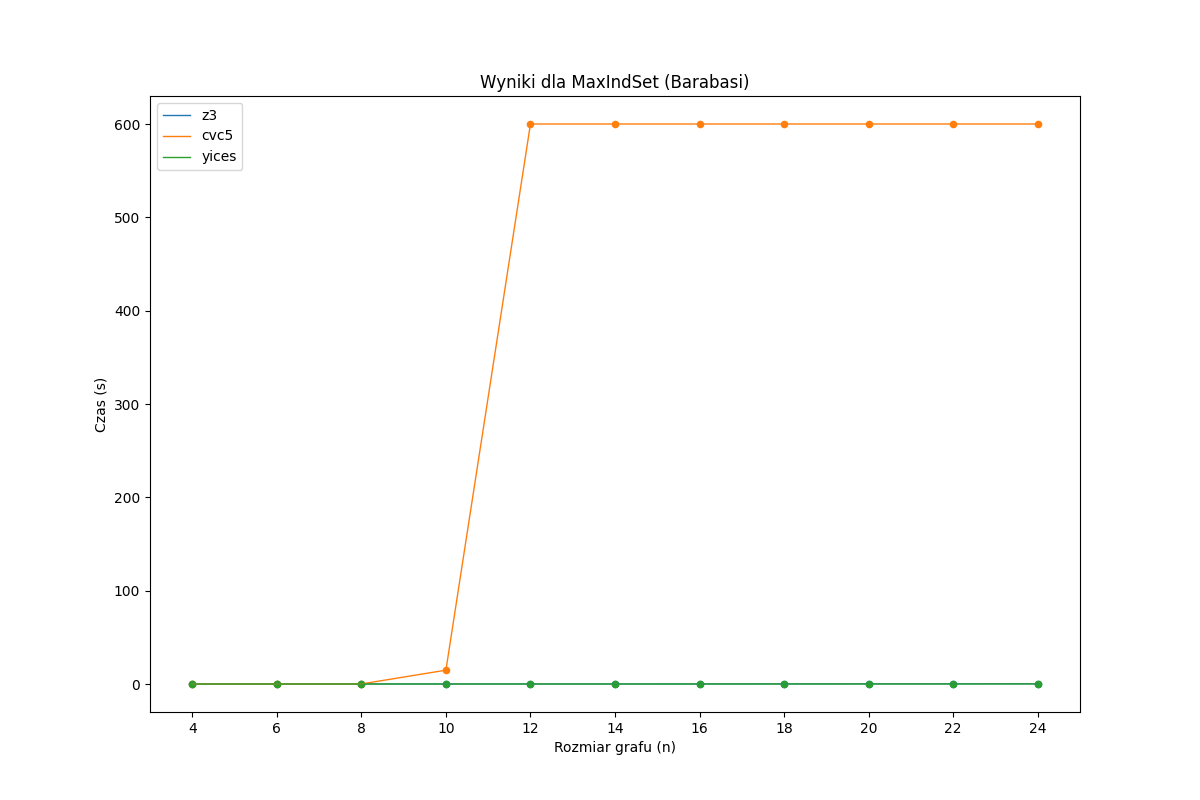
\includegraphics[width=\textwidth]{./figures/4-barabasi-plot.png}
		\caption{Wyniki eksperymentów dla grafów typu Barabási-Alberta.}
		\label{fig:4-barabasi-plot}
	\end{minipage}
\end{figure}

W przypadku grafów Erdős-Rényi, obserwowana sytuacja jest podobna do wyników uzyskanych dla grafów Barabási-Alberta. Niezależne zbiory w tych grafach były jeszcze mniejsze, co miało wpływ na szybkość działania solverów.

Z wykresu \ref{fig:4-erdos-renyi-plot} wynika, że zarówno Z3, jak i Yices, wykazywały błyskawiczną reakcję, udzielając odpowiedzi praktycznie natychmiastowo.

Natomiast CVC5 wykazał zmienność w swojej wydajności. Mimo że niektóre odpowiedzi udzielał szybko, od grafu z 10 wierzchołkami nagle zaczęły pojawiać się dłuższe czasy oczekiwania, a w przypadku niektórych instancji problemu czas działania przekroczył 10 minut.

\begin{figure}[htbp]
	\centering
	\begin{minipage}{\textwidth}
		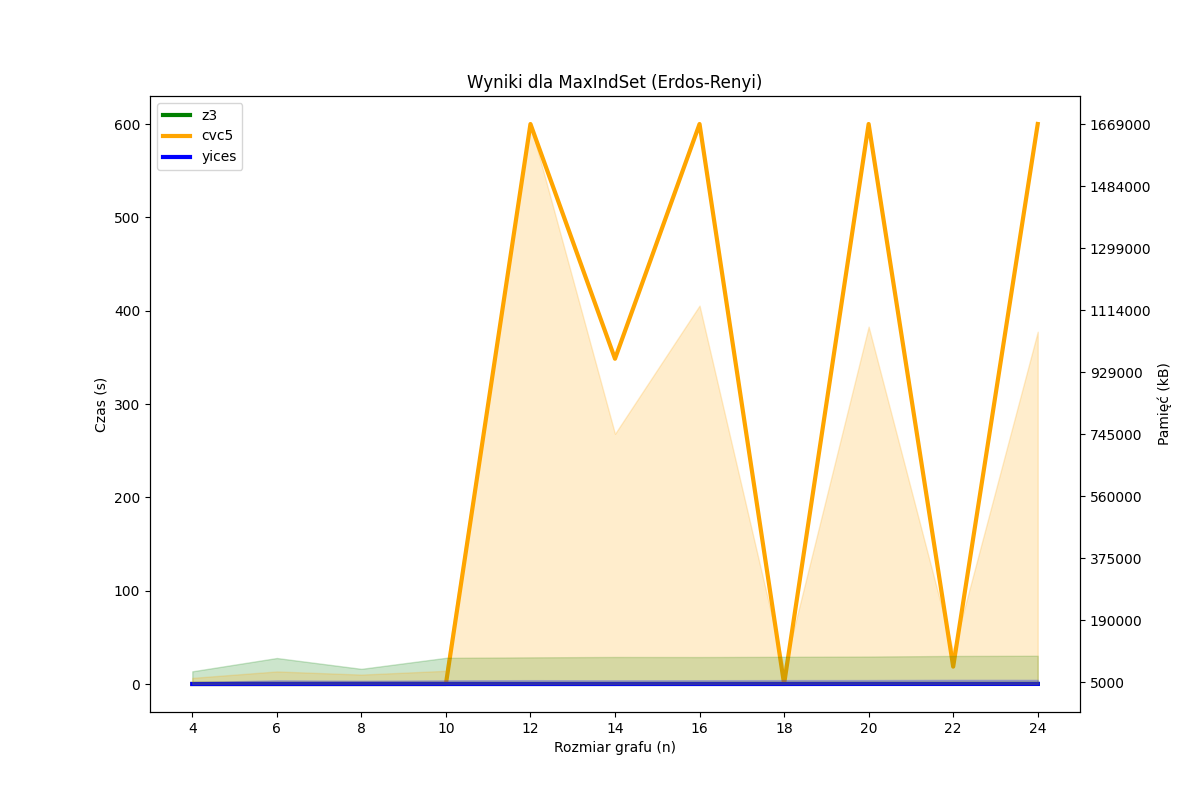
\includegraphics[width=\textwidth]{./figures/4-erdos-renyi-plot.png}
		\caption{Wyniki eksperymentów dla grafów typu Erdős-Rényi'ego.}
		\label{fig:4-erdos-renyi-plot}
	\end{minipage}
\end{figure}

Z tej analizy można wnioskować, że szybkość działania solverów Z3 i Yices jest prawdopodobnie związana z małymi rozmiarami niezależnych zbiorów zawartych w danych grafach. Na podstawie tych obserwacji można przypuszczać, że taka cecha znacząco ułatwia rozwiązanie problemu maksymalnego niezależnego zbioru. W kontekście naukowym taka hipoteza wskazuje na istotność rozmiaru zbioru w kwestii efektywnego przetwarzania problemów optymalizacyjnych.


\subsection{Wyniki dla Problemu pokrycia wierzchołkowego}

W wynikach eksperymentów dotyczących problemu pokrycia wierzchołkowego, wszystkie testowane solvery wykazywały zdolność do udzielania natychmiastowych odpowiedzi. Jednakże, interesujące różnice w wydajności można było zaobserwować w kontekście wykorzystania zasobów pamięci.

\begin{figure}[htbp]
	\centering
	\begin{minipage}{\textwidth}
		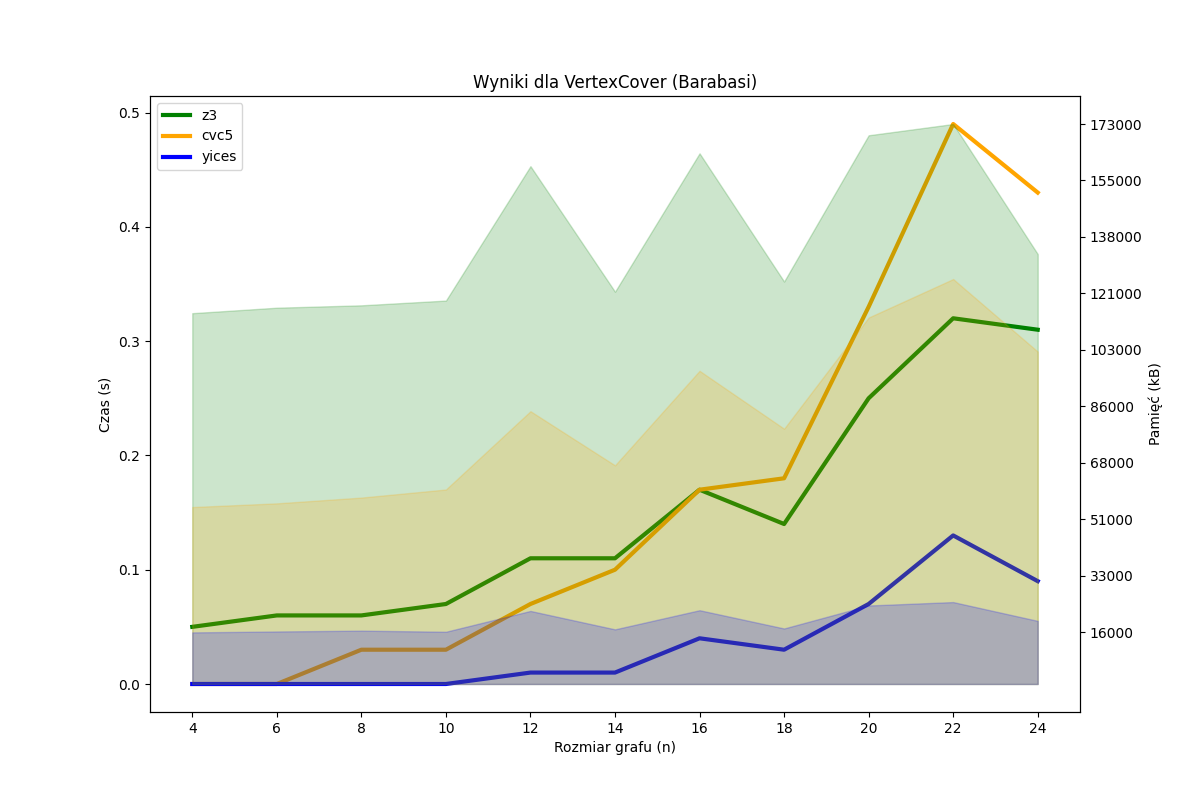
\includegraphics[width=\textwidth]{./figures/5-barabasi-plot.png}
		\caption{Wyniki eksperymentów dla grafów typu Barabási-Alberta.}
		\label{fig:5-barabasi-plot}
	\end{minipage}
\end{figure}

Analiza szczegółowych danych wykazała istotne różnice w szybkości działania oraz wykorzystaniu zasobów pamięci między solverami. Jak przedstawiono na wykresach \ref{fig:5-barabasi-plot} oraz \ref{fig:4-erdos-renyi-plot}, Yices wyróżniał się jako najszybszy spośród testowanych narzędzi dla obu typów grafów, udzielając odpowiedzi w bardzo krótkim czasie i wykorzystując dziesięciokrotnie mniej pamięci w porównaniu do pozostałych solwerów.

\begin{figure}[htbp]
	\centering
	\begin{minipage}{\textwidth}
		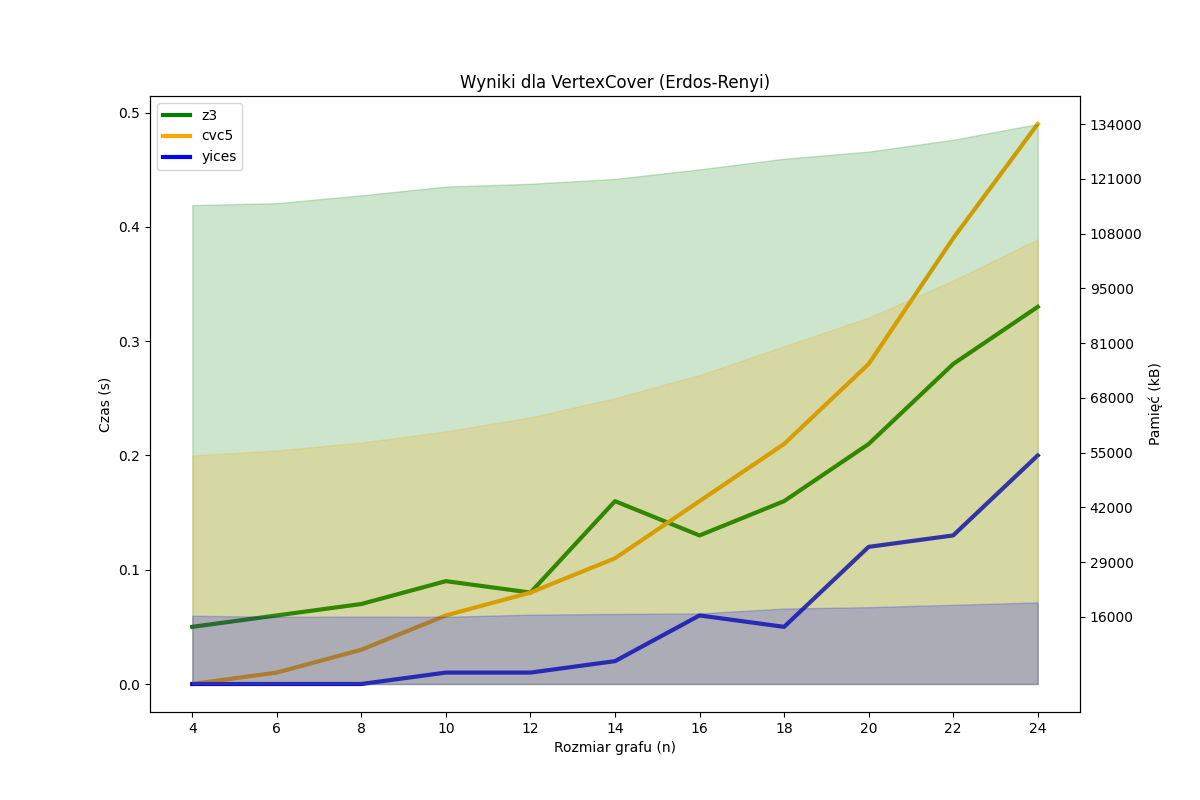
\includegraphics[width=\textwidth]{./figures/5-erdos-renyi-plot.png}
		\caption{Wyniki eksperymentów dla grafów typu Erdős-Rényi'ego.}
		\label{fig:5-erdos-renyi-plot}
	\end{minipage}
\end{figure}

Takie wnioski sugerują, że Yices może być szczególnie przydatny w przypadku problemów związanych z pokryciem wierzchołkowym, ze względu na swoją wydajność i oszczędne zarządzanie zasobami. 

\subsection{Wyniki dla Problemu kolorowania grafu}

Wyniki eksperymentów nad problemem kolorowania grafów wykazały znaczące różnice w wykorzystaniu zasobów pamięci przez różne solvery. Natomiast, zgodnie z wykresami \ref{fig:6-barabasi-plot} i \ref{fig:6-erdos-renyi-plot}, czas potrzebny na uzyskanie odpowiedzi był prawie taki sam dla wszystkich solverów. 

W przypadku, gdy nie było możliwości pokolorowania wszystkich wierzchołków (unsat), solvery szybko udzielały odpowiedzi, co sugeruje ich zdolność do efektywnego wykrywania niespełnionych ograniczeń.

\begin{figure}[htbp]
	\centering
	\begin{minipage}{\textwidth}
		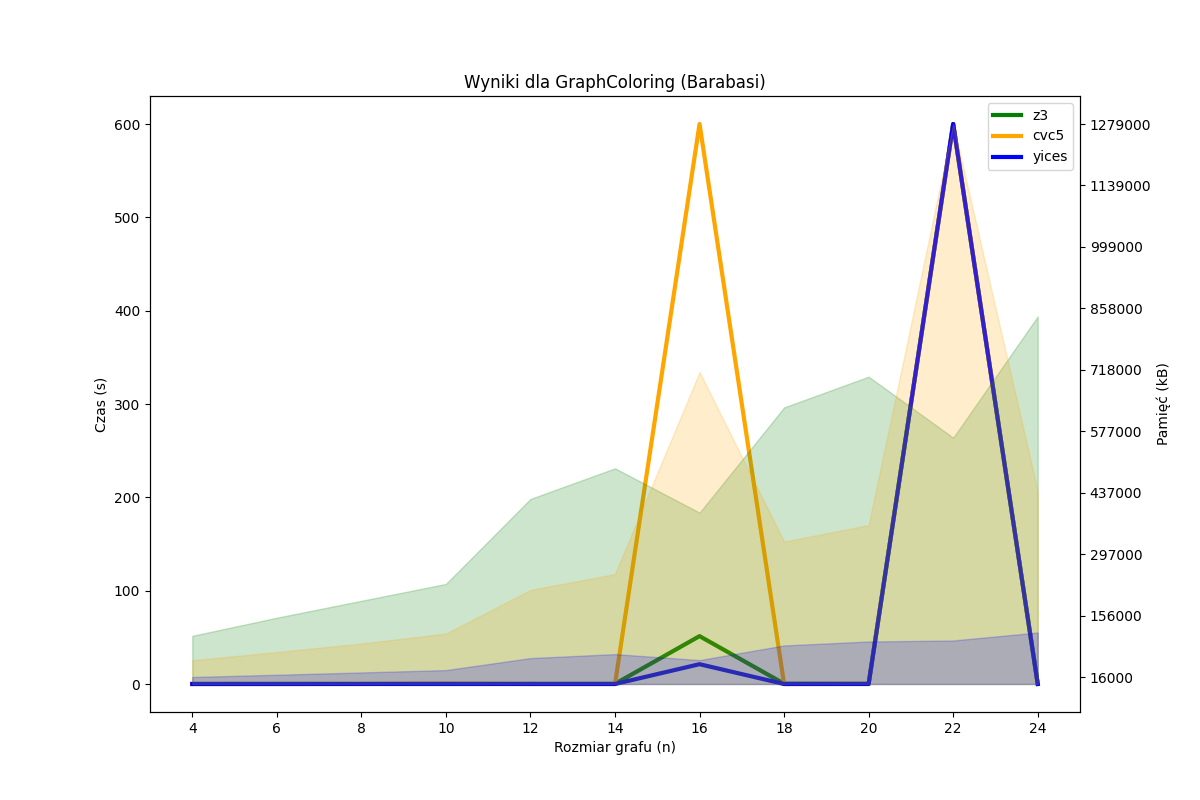
\includegraphics[width=\textwidth]{./figures/6-barabasi-plot.png}
		\caption{Wyniki eksperymentów dla grafów typu Barabási-Alberta.}
		\label{fig:6-barabasi-plot}
	\end{minipage}
\end{figure}

Jednakże, w sytuacjach, gdzie istniała możliwość pokolorowania grafu (sat), zaobserwowano wydłużenie czasu potrzebnego na uzyskanie odpowiedzi od solverów, zwłaszcza w przypadku, gdy liczba dostępnych kolorów była ograniczona. Im mniejsza liczba kolorów była potrzebna do pokolorowania grafu, tym dłużej solvery szukały odpowiedzi.

\begin{figure}[htbp]
	\centering
	\begin{minipage}{\textwidth}
		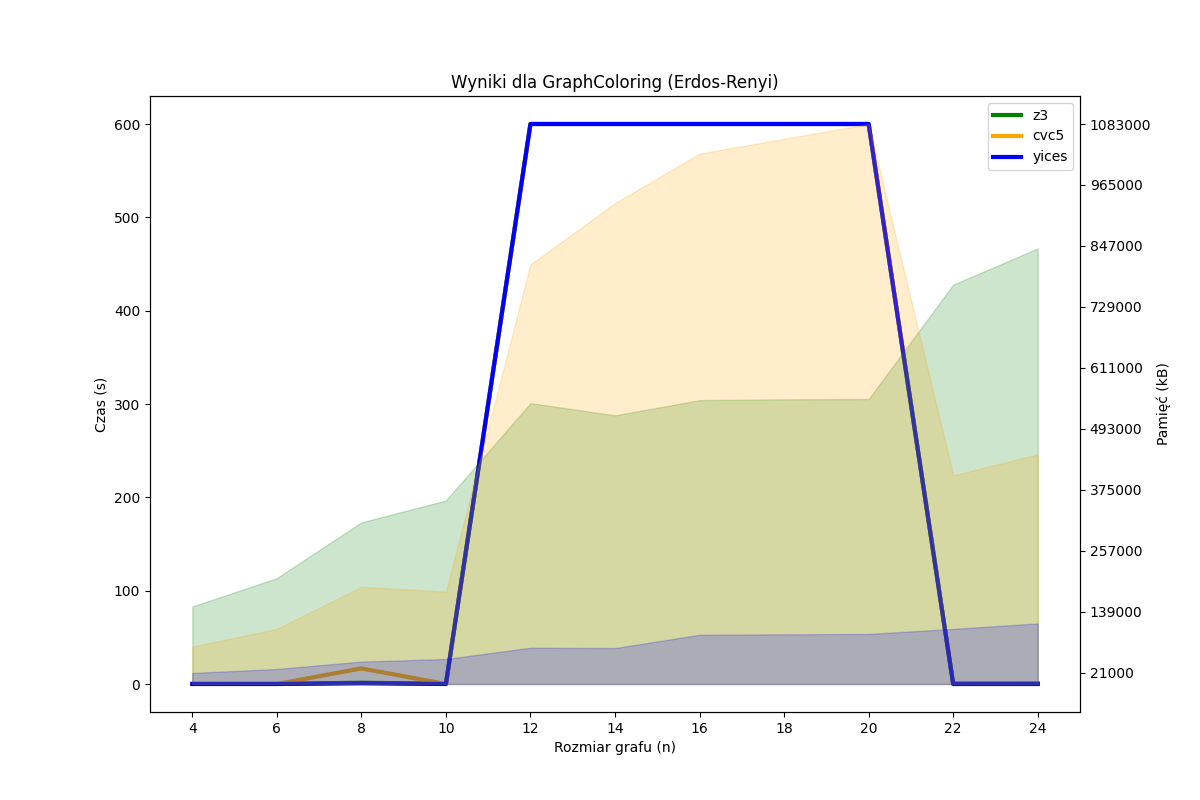
\includegraphics[width=\textwidth]{./figures/6-erdos-renyi-plot.png}
		\caption{Wyniki eksperymentów dla grafów typu Erdős-Rényi'ego.}
		\label{fig:6-erdos-renyi-plot}
	\end{minipage}
\end{figure}

Na podstawie danych z wykresu \ref{fig:6-erdos-renyi-plot} można stwierdzić, że CVC5 wyróżniał się potrzebą znacznie większej ilości pamięci w porównaniu do innych solverów, co wskazuje na jego ograniczenia w efektywnym zarządzaniu zasobami w przypadku tego konkretnego problemu kolorowania grafów.

\subsection{Wyniki dla Problemu Komiwojażera}

\subsection{Wyniki dla Problemu sumy podzbioru}

\section{Identyfikacja czynników wpływających na efektywność}

